\chapter{Proposed Methodology}
The Bicycle Management System is a smart project that automates bicycle rentals using a web platform. It applies object-oriented programming to manage users, track bicycles and handle reservations, making it ideal for learning real-world software development.

%This is for reference only. Delete before finalization


\section{Requirement Analysis \& Design Specification} The Bicycle Management System aims to simplify and digitize the process of renting, returning and tracking bicycles. During the requirement analysis, both functional and non-functional needs of the system were identified. Functional requirements include user registration, login authentication, viewing available bicycles, booking and returning cycles. Admin-specific features include managing bicycle inventory, tracking usage and viewing system reports.\\
The design specification phase focused on building a structured system using object-oriented principles, with clear definitions of classes such as User, Admin, Bicycle, and Booking. The system was designed with a responsive user interface and a MySQL database for reliable data storage and retrieval. Security, scalability and ease of use were also key considerations to ensure the system performs well in real-world environments like campuses or public bike-sharing programs.
\cite{2.1.1}

\subsection{Overview}
The diagram for the Bicycle Management System illustrates a basic web-based platform that allows users to manage bicycle rentals efficiently. Users interact with the system through a login portal, where they can view available bicycles, book a ride and return bicycles after use.\\
The system processes these actions using a backend database, typically MySQL, which handles data related to users, bicycles and bookings. Object-oriented components such as User, Bicycle, and Reservation classes interact to maintain smooth operations.\\
This project offers an easy and user-friendly way to handle bike-sharing tasks, promoting organized, hands-free management through a digital interface.\cite{2.1.3}

\subsection{Proposed Methodology}
\begin{itemize}
\item \textbf{User Interaction:} Users access the system through a web interface where they can register, log in and manage their bicycle rentals.
\item \textbf{Data Processing:} Once a user makes a request (such as booking a bicycle), the system processes it using backend logic implemented with object-oriented programming concepts.
\item \textbf{Database Management:} The system uses a MySQL database to store and retrieve data related to bicycles, users and bookings. All interactions are logged and updated in real-time for accuracy.
\item\textbf{Booking Confirmation:} When a booking is confirmed, the system updates the bicycle’s status and ensures it is marked as unavailable until returned.
\item \textbf{System Hosting: } The application runs on a local server or web host, supported by a stable backend framework and database connection, ensuring smooth and efficient operation of all modules.\cite{2.1.1}
\end{itemize}

\begin{figure}[h] % 'h' for placing it "here"
\subsection{UML Design}
    \centering
    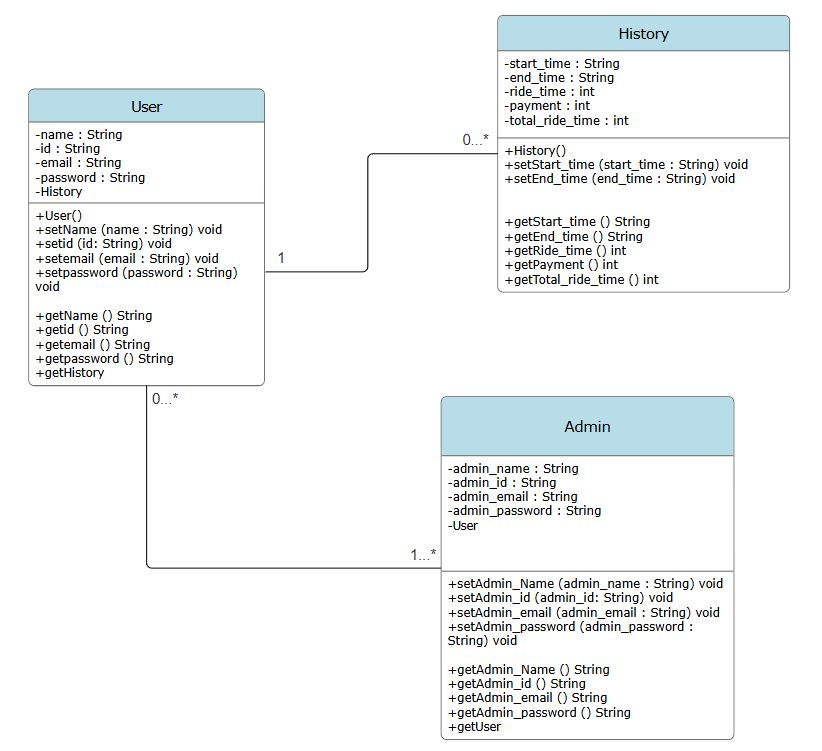
\includegraphics[width=0.9\textwidth]{figures/Others/UML.jpg} % Replace 'UML.jpg' with your image file
    \caption{UML}
    \label{fig:sample}
\end{figure}


\subsection{Frontend Design}
\begin{figure}[H]
    \centering
    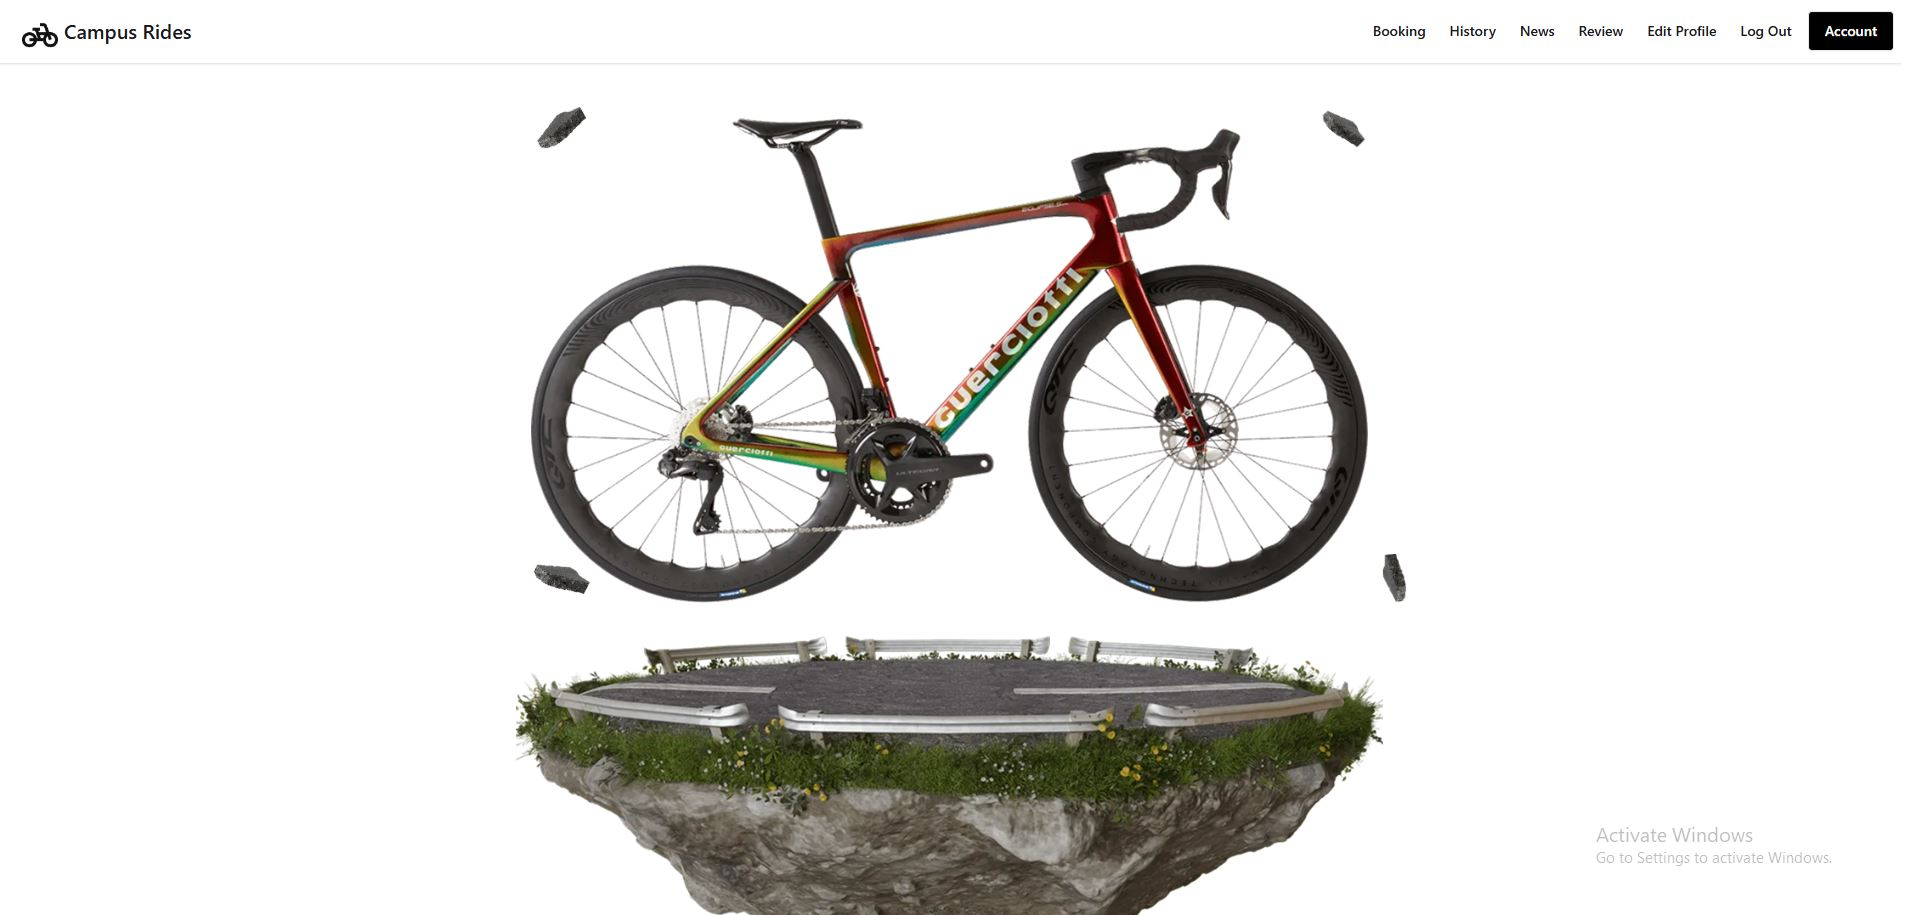
\includegraphics[width=0.6\textwidth]{figures/UI/home.jpg} % Replace with your image path
    \caption{Home Page}
    \label{fig:sample}
\end{figure}
\begin{figure}[H]
    \centering
    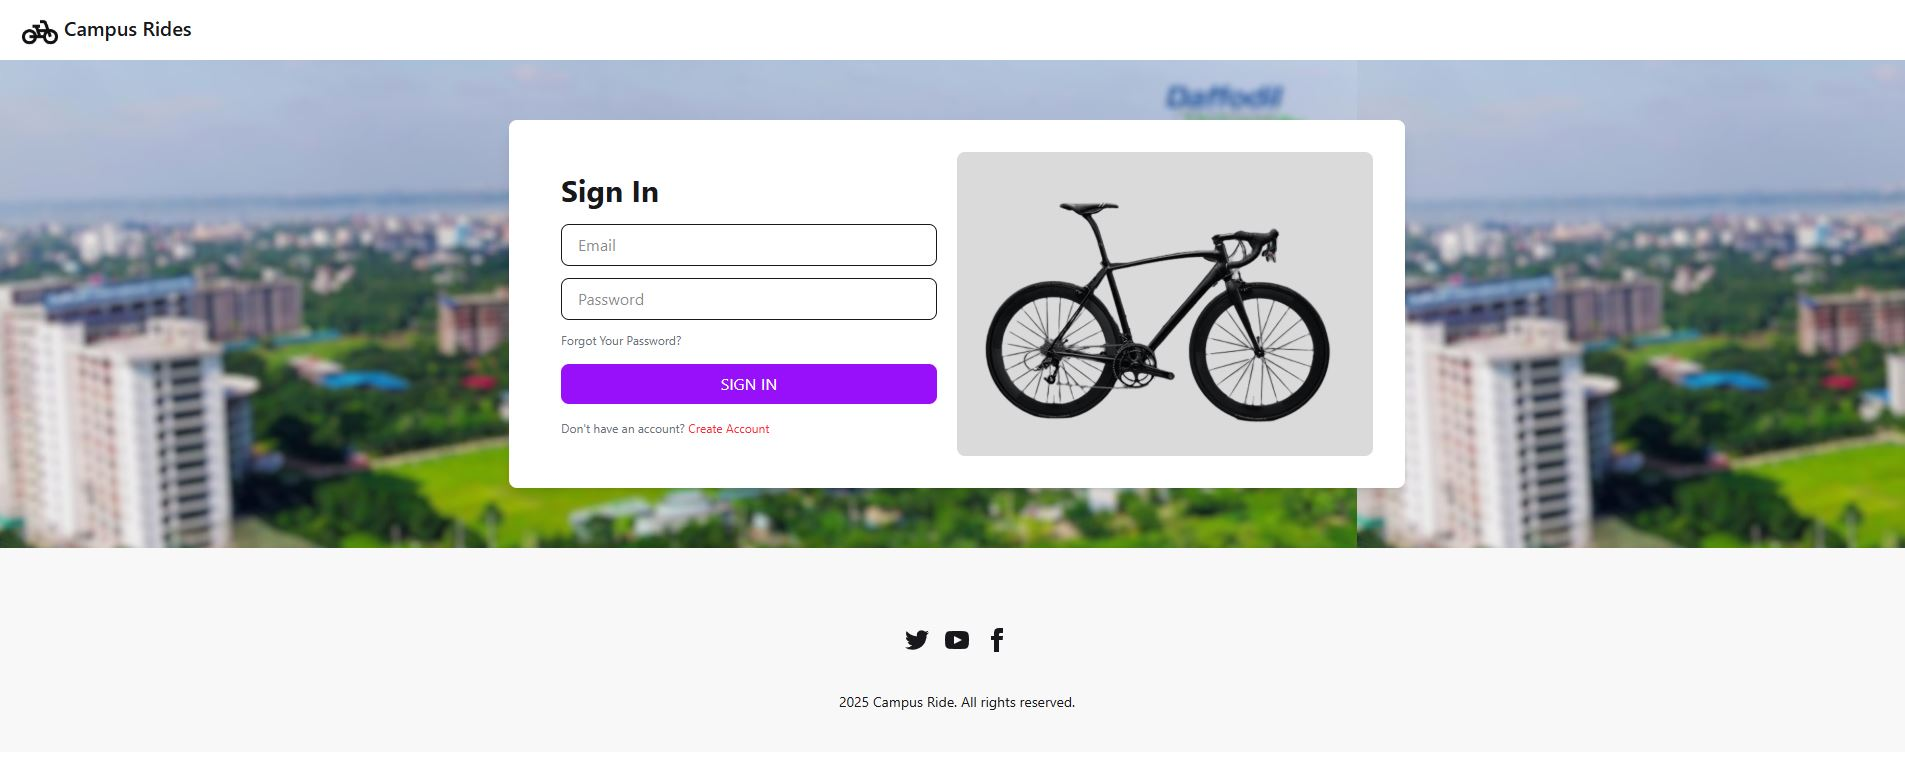
\includegraphics[width=0.6\textwidth]{figures/UI/log_in.jpg} % Replace with your image path
    \caption{Login Page}
    \label{fig:sample}
\end{figure}
\begin{figure}[H]
    \centering
    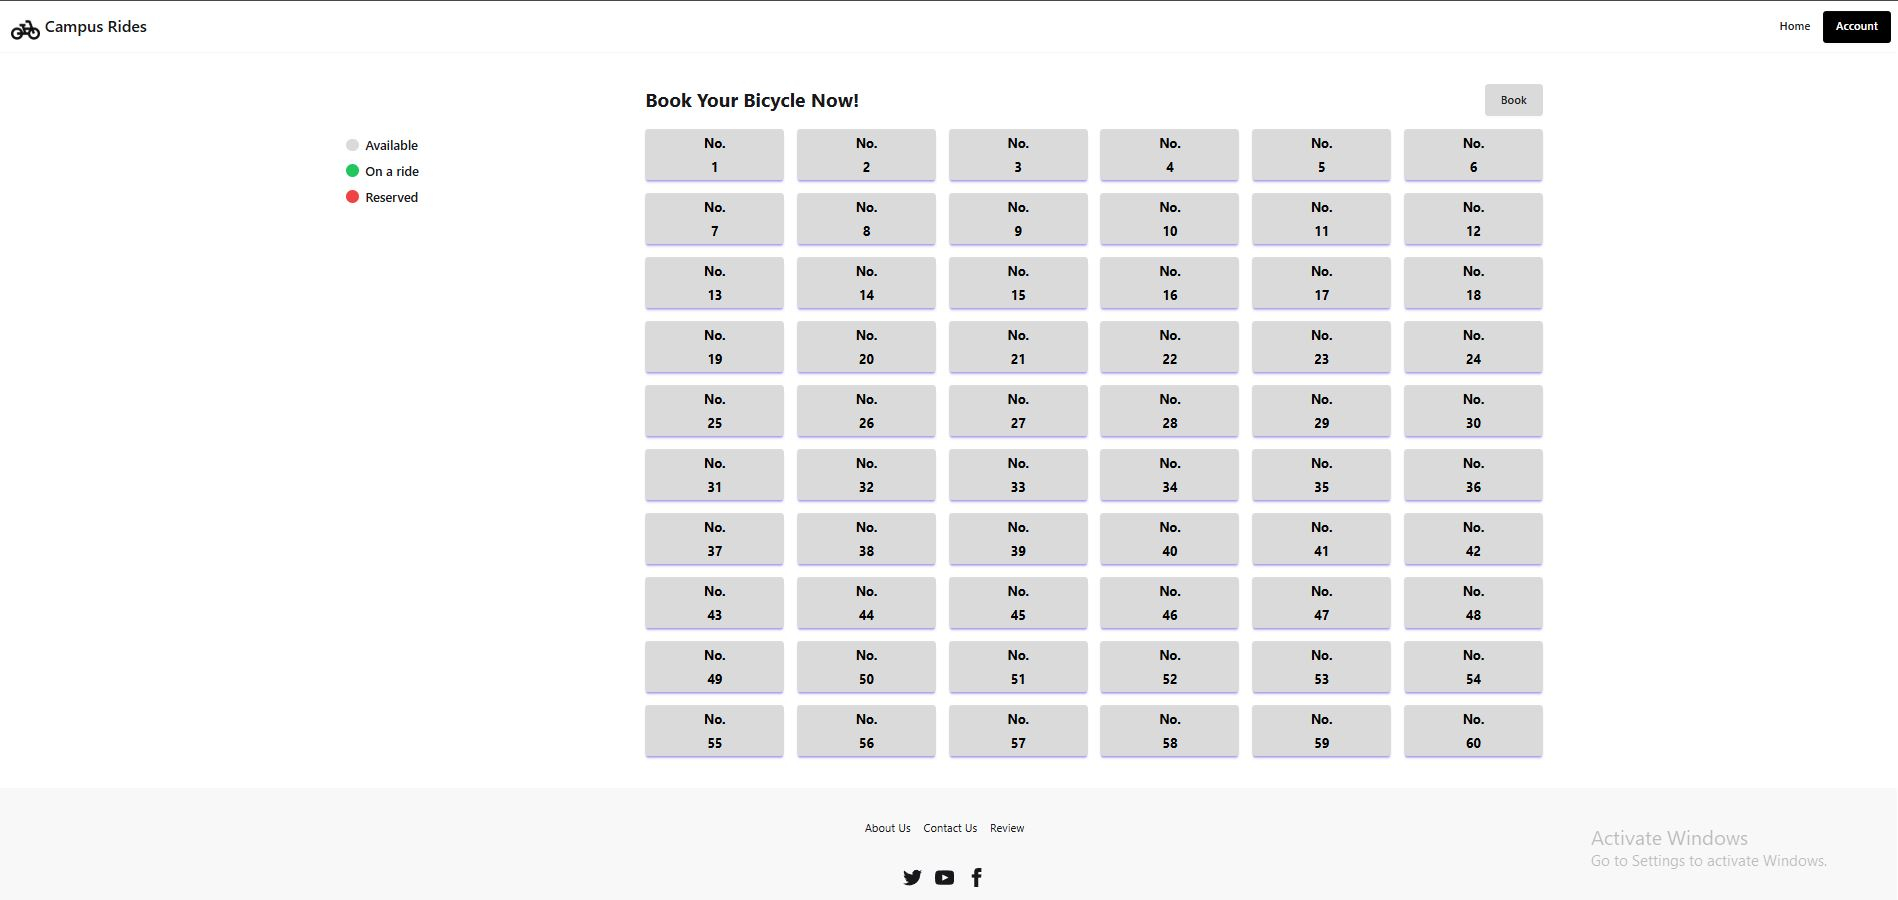
\includegraphics[width=0.5\textwidth]{figures/UI/booking.jpg} % Replace with your image path
    \caption{Booking Page}
    \label{fig:sample}
\end{figure}
\begin{figure}[H]
    \centering
    \includegraphics[width=0.9\textwidth]{figures/UI/timer.jpg} % Replace with your image path
    \caption{Timer Page}
    \label{fig:sample}
\end{figure}
\begin{figure}[H]
    \centering
    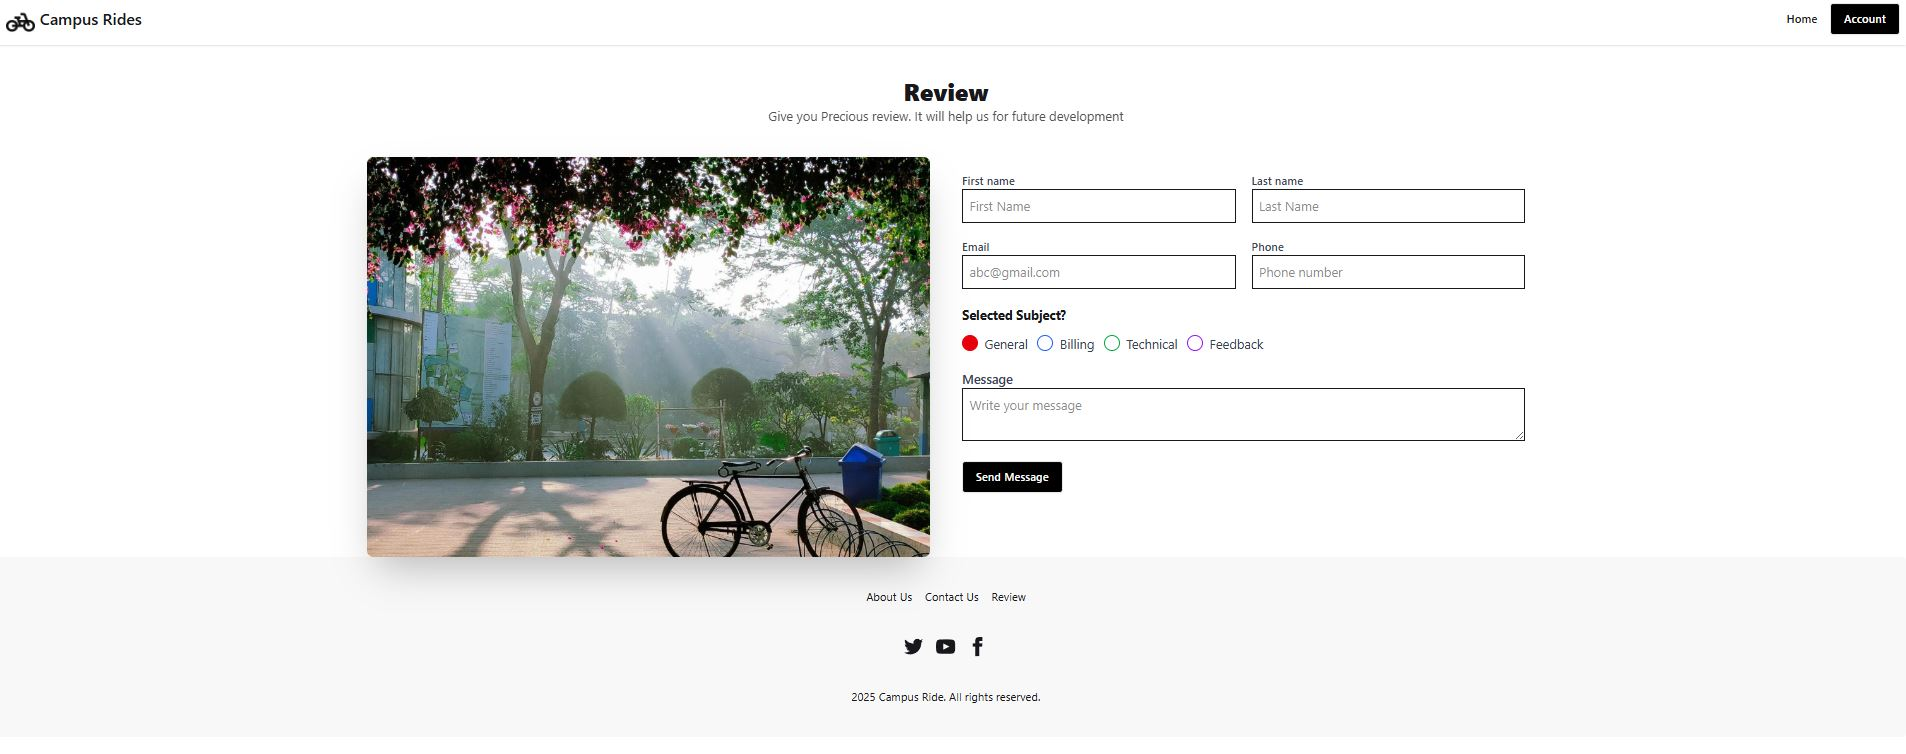
\includegraphics[width=0.7\textwidth]{figures/UI/review.jpg} % Replace with your image path
    \caption{Review Page}
    \label{fig:sample}
\end{figure}
    
\section{Overall Project Plan}
The Bicycle Management System Project focuses on creating a web-based platform to efficiently manage shared bicycles. The project will move through phases including research, design, hardware selection, web development, testing and improvement based on user feedback.\\

\noindent The system will use components like GPS modules, RFID/NFC tags and microcontrollers to monitor bicycle location and usage. A web application will be developed to handle user registration, bicycle tracking and real-time status updates.\\

\noindent All management functions such as checking availability, assigning bicycles  and viewing usage history will be accessible through the web interface. Testing will ensure the system is accurate, secure and user-friendly. The goal is to deliver a practical and reliable bicycle management solution without relying on mobile apps.\cite{2.2}\\

\begin{table}[h!]
\subsection{Time Frame}
\centering
\begin{tabular}{|l|c|c|c|c|}
\hline
\textbf{Working Days}              & \textbf{Analysis+Content Ready} & \textbf{Frontend} & \textbf{DataBase} & \textbf{Backend} \\ \hline
Week 1 & \checkmark              &                 &                 &                 \\ \hline
Week 2             & \checkmark            &  \checkmark               &                 &                 \\ \hline
Week 3        &               &  \checkmark               &                 &   \checkmark               \\ \hline
Week 4        &                &              & \checkmark                 &    \checkmark              \\ \hline
Week 5        &                &              &   \checkmark               &   \checkmark               \\ \hline
Week 6      &                &                 & \checkmark              &   \checkmark               \\ \hline
\end{tabular}
\caption{Project Schedule.}
\label{tab:project_schedule}
\end{table}

